\chapter{Introduction}
\section{Problem Statement}
The dataset is related to red variants of the Portuguese "Vinho Verde" wine.The dataset describes the amount of various chemicals present in wine and their effect on it's quality. The datasets can be viewed as classification or regression tasks. The classes are ordered and not balanced (e.g. there are much more normal wines than excellent or poor ones).Task is to predict the quality of wine using the given data.

A simple yet challenging project, to anticipate the quality of wine.

The complexity arises due to the fact that the dataset has fewer samples, \& is highly imbalanced.

\textbf{Data Source} : \href{https://archive.ics.uci.edu/ml/datasets/wine+quality}{https://archive.ics.uci.edu/ml/datasets/wine+quality}

\section{About Dataset}
The dataset contains the following columns:
\begin{enumerate}
    \item fixed acidity
    \item volatile acidity
    \item citric acid
    \item residual sugar
    \item chlorides
    \item free sulfur dioxide
    \item total sulfur dioxide
    \item density
    \item pH
    \item sulphates
    \item alcohol
    \item quality (Targe Variable) : ranges from 0 to 10
\end{enumerate}

The data information is as follow:
\begin{figure}[H]
    \centering
    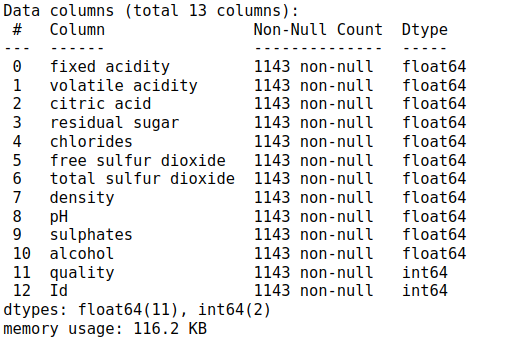
\includegraphics[scale = 0.7]{data_info.png}
    \caption{Data Information}
    \label{fig:Data Information}
\end{figure}

Description of each column is shown below:

\begin{table}[H]
    \begin{center}
        \begin{tabular}{ |c|c|c|c|c|c|c| }
            \hline
            stats      & 
            fixed acidity&	volatile acidity	&citric acid&	residual sugar&	chlorides	&free sulfur dioxide  \\
            \hline
            mean & 8.311	& 0.5313	& 0.264 &	2.532 &	0.0869	& 15.615 \\
            \hline

            std & 1.747	&0.179&	0.196&	1.355	&0.0477&	10.250 \\
            \hline

            min & 4.600&	0.120000	&0.000&	0.900	&0.0120&	1.00 \\
            \hline

            25\% & 7.100	&0.39250 & 0.0900 &	1.900	&0.070&	7.000 \\
            \hline

            50\% & 7.900 &	0.5200&0.2500	&2.200&	0.0790&13.000	 \\
            \hline

            75\% & 9.100	&0.6400&0.4200&2.6000&0.090	&21.000	 \\
            \hline

            max & 15.900 &	1.580	&1.00&	15.50&	0.6110	&68.00 \\
            \hline
        \end{tabular}
    \end{center}
    \caption{Data Description 1}
    \label{table:Data Description 1}
\end{table}


\begin{table}[H]
    \begin{center}
        \begin{tabular}{ |c|c|c|c|c|c| }
            \hline
            stats      & 
            total sulfur dioxide	&density&	pH	&sulphates&	alcohol	  \\
            \hline
            mean & 45.914698	&0.996730&	3.311015	&0.657708	&10.442111 \\
            \hline

            std & 32.782130	&0.001925&	0.156664&	0.170399&	1.082196	\\
            \hline

            min & 6.000000	&0.990070	&2.740000&	0.330000	&8.400000	 \\
            \hline

            25\% & 21.000000	&0.995570&	3.205000	&0.550000&	9.500000	 \\
            \hline

            50\% & 37.000000	&0.996680&	3.310000	&0.620000&	10.200000		 \\
            \hline

            75\% & 61.000000&	0.997845&	3.400000&	0.730000&	11.100000		 \\
            \hline

            max & 289.000000 &	1.003690&	4.010000&	2.000000&	14.900000	 \\
            \hline
        \end{tabular}
    \end{center}
    \caption{Data Description 2}
    \label{table:Data Description 2}
\end{table}



\section{Dataset Statistics}
The count plot of the whole dataset on the basis of quality of wine is shown below.

\begin{figure}[H]
    \centering
    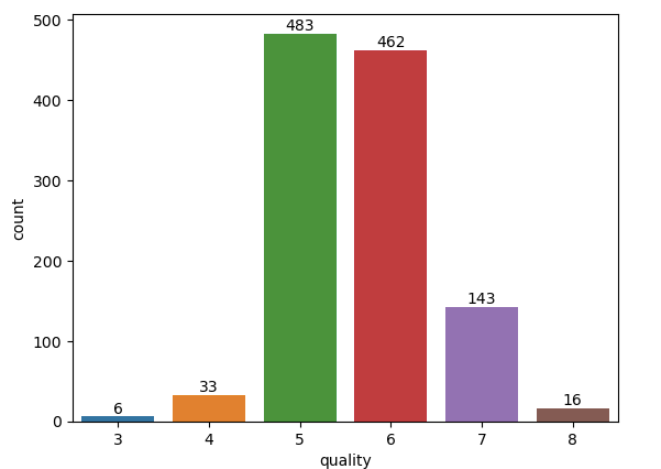
\includegraphics[scale = 0.7]{whole_dataset_countplot.png}
    \caption{Quality Count plot}
    \label{fig:Quality Count plot}
\end{figure}

We can see from above countplot, that the data is highly imbalanced and quality of wine(0, 1, 2, 9, 10) are not present in the dataset.

In order to deal with this imbalanced, at first we are going to merge the quality labels (3 and 4) and (7 and 8) as shown below.


\begin{figure}[H]
    \centering
    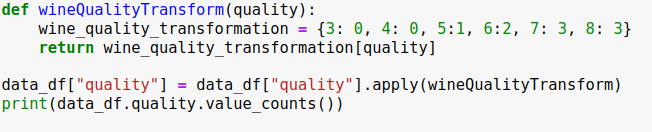
\includegraphics[scale = 0.7]{wineQualityTransformCode.png}
    \caption{Code for transformation of quality attribute}
    \label{fig:Code for transformation of quality attribute}
\end{figure}

The resulting count plot is as shown below:
\begin{figure}[H]
    \centering
    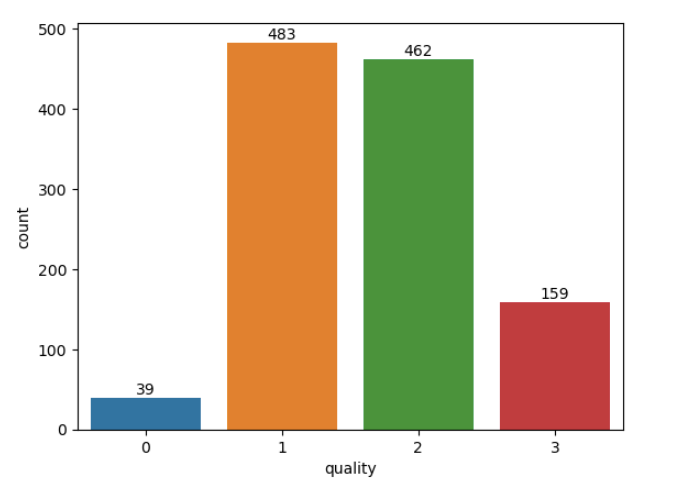
\includegraphics[scale = 0.7]{transformed_whole_dataset_countplot.png}
    \caption{Quality Count plot after transformation}
    \label{fig:Quality Count plot after transformation}
\end{figure}

\subsection{Train, validation and test dataset}
We are going to use 80\%, 20\% and 20\% of the dataset as training, validation and test data. The countplot are as shown below:

\begin{figure}[H]
    \centering
    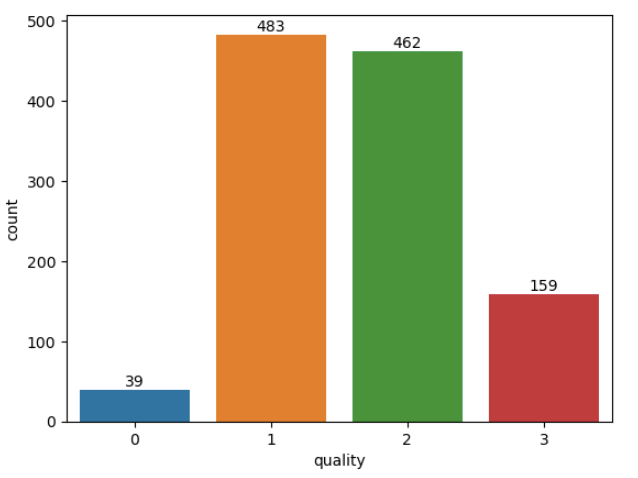
\includegraphics[scale = 0.7]{train_count_plot.png}
    \caption{Train Quality Count plot after transformation}
    \label{fig:Train Quality Count plot after transformation}
\end{figure}

\begin{figure}[H]
    \centering
    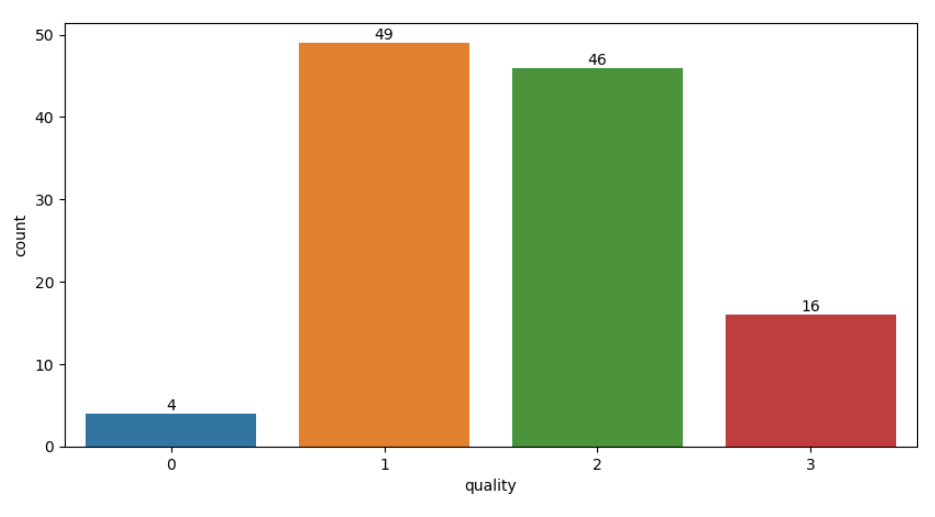
\includegraphics[scale = 0.5]{val_count_plot.png}
    \caption{Validation Quality Count plot after transformation}
    \label{fig:Validation Quality Count plot after transformation}
\end{figure}

\begin{figure}[H]
    \centering
    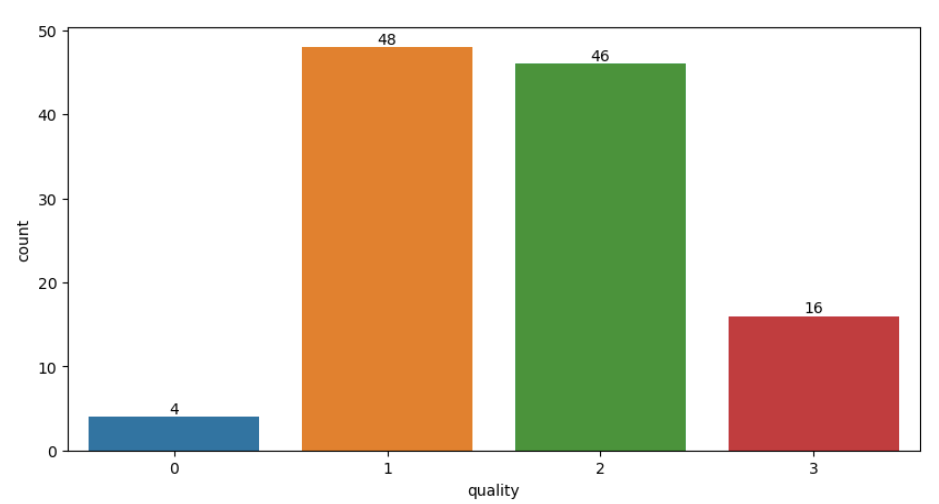
\includegraphics[scale = 0.5]{test_count_plot.png}
    \caption{Test Quality Count plot after transformation}
    \label{fig:Test Quality Count plot after transformation}
\end{figure}

\section{Expected Outcome}
We expect the output to be the list of probabilites of belonging to a class[0, 1, 2 or 3]. Among these, the class with higher probability is out predicted class.

